%*----------- SLIDE -------------------------------------------------------------
\begin{frame}[t]{Introduction}    
  \transdissolve[duration=0.5]
  The main objective of this research is to propose an AUV model with small dimensions, capable of carrying missions on sea coastal and shallow waters with 50 meters deep. 

  For this project, is expected: 
  \newline
  \begin{columns}[c]
    \column{.05\textwidth}
    \column{.6\textwidth}
      \begin{enumerate}
        \item A navigation system able to navigate in indoor and outdoor environments
        \item Identify and avoid objects
        \item Perform all activities with minimal intervention
      \end{enumerate}
    \column{.35\textwidth}
      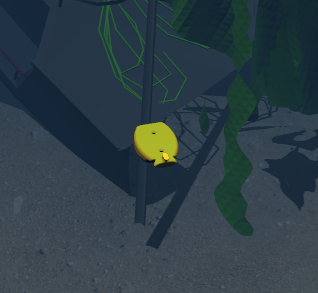
\includegraphics[width=1\textwidth]{turbot_intro.png}
  \end{columns}

%*----------- notes
  \note[item]{Notes can help you to remember important information. Turn on the notes option.}
\end{frame}
%*----------- SLIDE -------------------------------------------------------------
\begin{frame}[t]{Main requirements}
  \transdissolve[duration=0.5]
  \begin{columns}[c]
    \column{.5\textwidth}
      \textbf{Customer}
      \begin{itemize}
        \item Indoor/outdoor navigation
        \item Obstacle avoidance
        \item Autonomous navigation
        \item Small dimensions
        \item Energetic efficiency
        \item Lighting system
      \end{itemize}
    \column{.5\textwidth}
      \textbf{System}
      \begin{itemize}
        \item 5 DOF and 6 Thrusters composition
        \item Perceive dynamic environments
        \item Max 0,8 x 0,5 x 0,5 m dimentions
        \item Max 20 kg weight
        \item 2 h of battery autonomy
        \item Positive buoyancy
      \end{itemize}
  \end{columns}
\end{frame}

%*----------- SLIDE -------------------------------------------------------------
\begin{frame}[t]{Working environments}
  \transdissolve[duration=0.5]
  \begin{columns}[c]
    \column{.5\textwidth}
      turBOT is capable to navigate in indoor or outdoor environments but is being developed for coastal sea 50 m deep. 
    \column{.5\textwidth}
      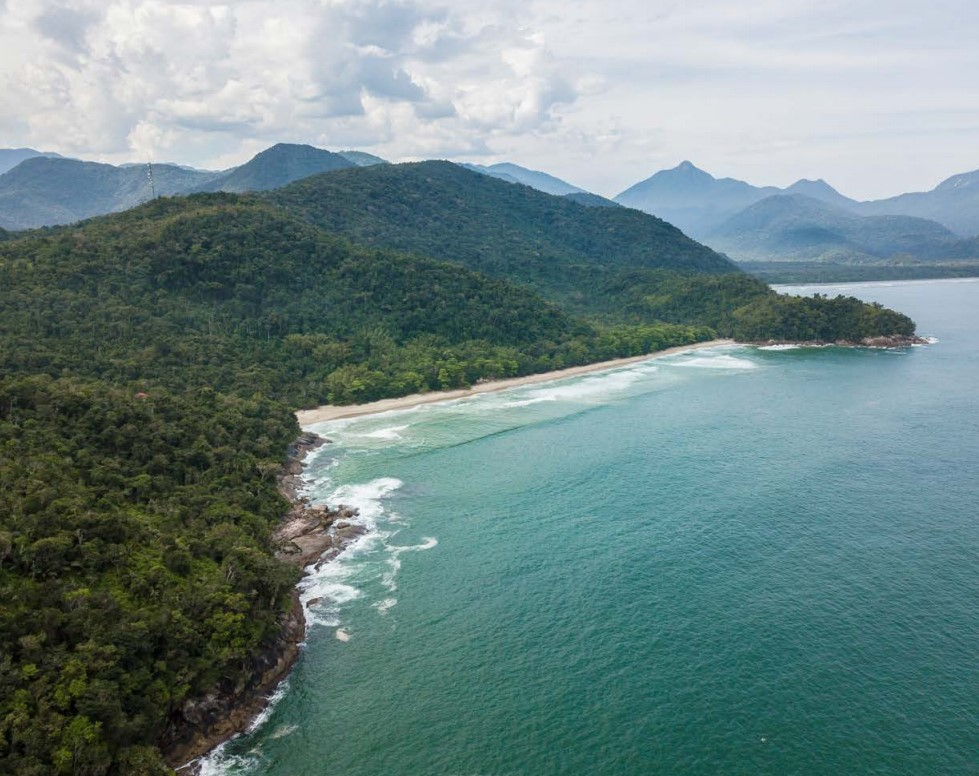
\includegraphics[width=.85\textwidth]{coastal.jpg}
  \end{columns}
\end{frame}

%*----------- SLIDE -------------------------------------------------------------
\begin{frame}[t]{Vehicle's design}
  \transboxout[duration=0.5]
  \begin{columns}
    \column{.0\textwidth}
    \column{.5\textwidth}
      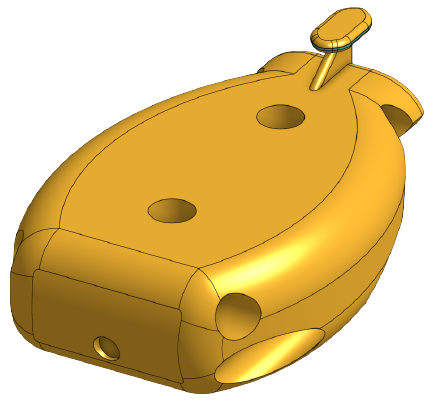
\includegraphics[width=.85\textwidth]{turbot_design.png}
    \column{.5\textwidth}
      The first vehicle's design was made using OnShape software,based on real-life Turbot Fish. 

      After CFD analysis, an optimized design a will be developed by the team.
        % \begin{enumerate}
        %     \item plataforma antropormórfica Darwin-OP;
        %     \item 20 DoF\footnote{do inglês, graus de liberdade};
        %     \item composto de 18 servo-motores;
        %     \item possui um grande gama de sensores para interação.
        % \end{enumerate}
  \end{columns}
%*----------- notes
  \note[item]{Notes can help you to remember important information. Turn on the notes option.}
\end{frame}
%*----------- SLIDE -------------------------------------------------------------
\begin{frame}[t]{Vehicle's dimensions}
  \centering
  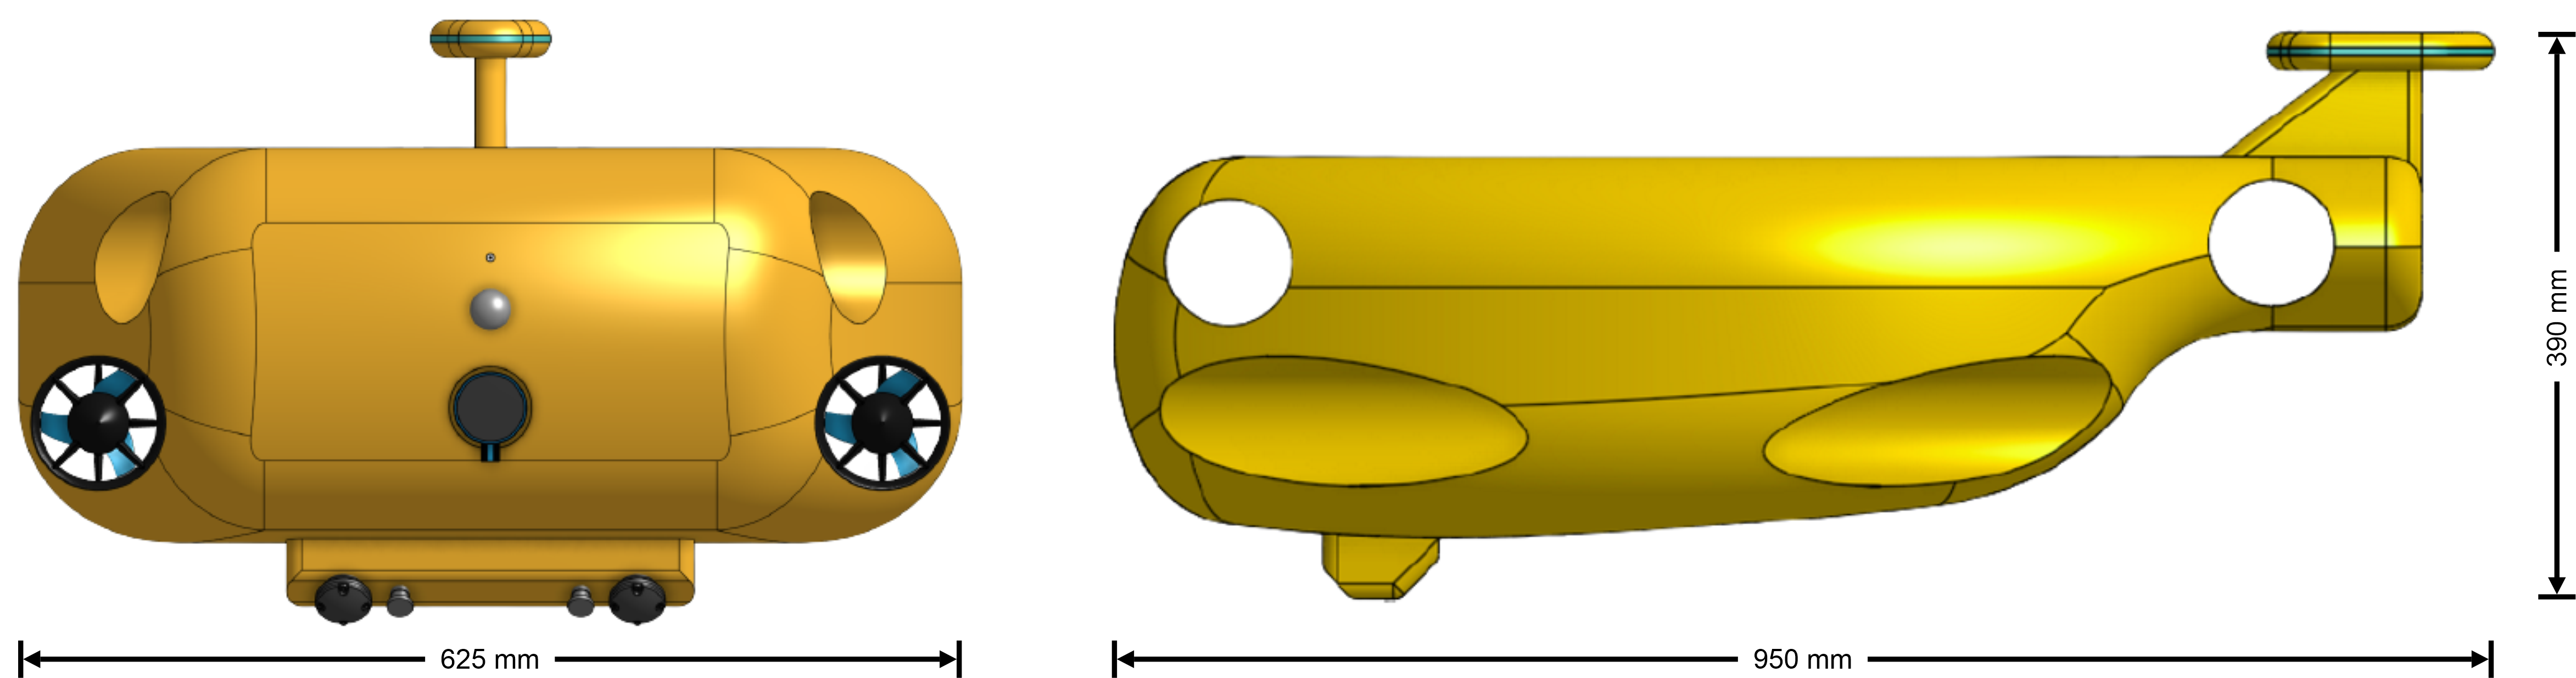
\includegraphics[width=1.0\textwidth]{dimensions.png}  
\end{frame}

%*----------- SLIDE -------------------------------------------------------------
\begin{frame}[c]{Sensors and peripherals}
  \transboxout[duration=0.5]
  In order for the AUV to act autonomously, these sensors and general peripherals were chosen:
  \begin{columns}
    \column{.02\textwidth}
    \column{.48\textwidth}
      \begin{enumerate}
        \item Low-light HD USB camera
        \item Minteye standard stereo camera
        \item Ping sonar altimeter and echosounder
        \item Red laser diode module
        \item MPU6050 IMU
        \item Venus638Flpx GPS
        \item Lumen Subsea Light
      \end{enumerate}
    \column{.4\textwidth}
      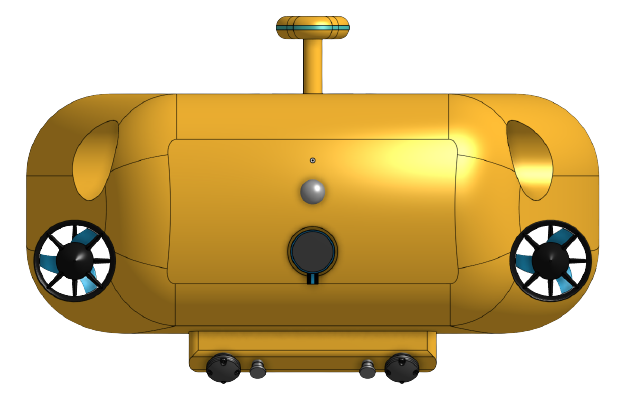
\includegraphics[width=1.0\textwidth]{turbot_front.png}      
  \end{columns}
\end{frame}


%*----------- SLIDE -------------------------------------------------------------
\begin{frame}[c]{Resultant force between weight x buoyancy}
  Values such as weight, volume and center of mass are reported by OnShape. The resulting force between the weight and the buoyancy found through this formula:
  
  \begin{equation} 
    F_{r} = a_{g}(\rho_{f} V_{s} - m_{v})
  \end{equation}
  \begin{columns}
    \column{.5\textwidth}
      \begin{itemize}
        \item $a_{g} =$ Gravity acceleration
        \item $\rho_{f} =$ Fluid density
        \item $V_{s} =$ Submerged volume
        \item $m_{v} =$ Vehicle's mass
      \end{itemize}
    \column{.5\textwidth}
      turBOT data calc: \\
      $F_{r} = a_{g}(\rho_{f} V_{s} - m_{v})$ \\
      $F_{r} = 9.8 \frac{m}{s^2}(1028 \frac{kg}{m^3}* 0.016 m^3 - 17 kg)$ \\
      $F_{r} = 1.64 N$
  \end{columns}
  
  It is ideal if the buoyancy is slightly positive so that the vehicle floats and at the same time can dive without much effort from the thrusters.  
\end{frame}

%*----------- SLIDE -------------------------------------------------------------
\begin{frame}[c]{Drag force}
  In order to minimize thruster effort, it is important to develop a structure that results in a minimal drag force. This force can be calculated through this formula:   
  
  \begin{equation}
    D = -\frac{1}{2}C_{d} \rho_{f} A v^2
  \end{equation}
  \begin{columns}
    \column{.5\textwidth}
      \begin{itemize}
        \item $C_{d} =$ Drag coefficient
        \item $\rho_{f} =$ Fluid density
        \item $A =$ Transversal area or cross sectional area
        \item $v =$ Relative velocity   
      \end{itemize}
    \column{.5\textwidth}
    Front: \\
      $D = -\frac{1}{2} * 0.42 * 1028 \frac{kg}{m^3} * 0.164 m^2 * 1 \frac{m^2}{s^2}$ \\
      $D = 35.49 N$ \\
    Side: \\
      $D = -\frac{1}{2} * 0.42 * 1028 \frac{kg}{m^3} * 0.275 m^2 * 0.5 \frac{m^2}{s^2}$ \\
      $D =  14.34 N$
  \end{columns}
  

\end{frame}

%*----------- SLIDE -------------------------------------------------------------
\begin{frame}[c]{Battery autonomy}
  For the calculation of the battery autonomy, it was considered that the vehicle stays stable at the same depth and move forward and laterally at 1.0 m/s and 0.5 m/s.
  
  % \begin{columns}
  %   \column{.5\textwidth}
  %     % \begin{itemize}
  %     %   \item Stays stable at the same depth
  %     %   \item Moves forward at a speed of 1.0 m/s
  %     %   \item Moves laterally at a speed of 0.5 m/s
  %     % \end{itemize}
  %   \column{.5\textwidth}
  %     According to the calculations, using 2 batteries 36 Ah, turBOT works for 2.14 hours.
  % \end{columns}

  \begin{columns}
    \column{.5\textwidth}
      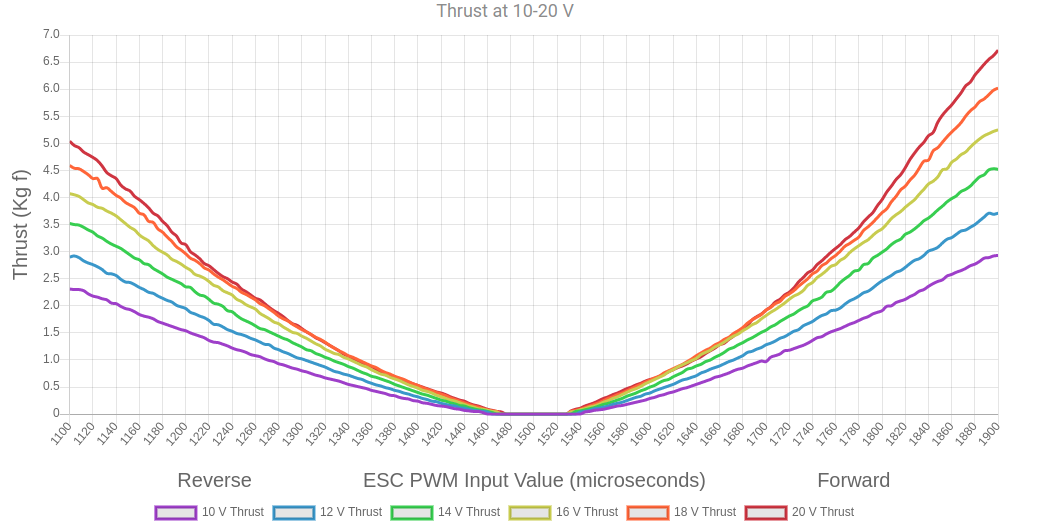
\includegraphics[width=1.0\textwidth]{thrust_graph.png}
    \column{.5\textwidth}
      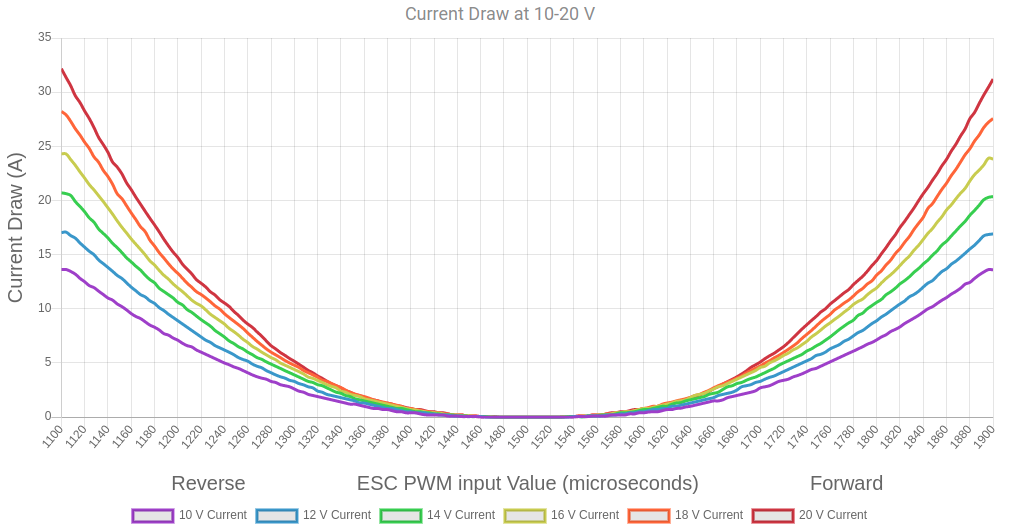
\includegraphics[width=1.0\textwidth]{current_graph.png}
  \end{columns}

  The current that each thruster will require for them to exert the necessary force was obtained. Using 2 batteries 18 Ah, battery life of 2.14 hours could be estimated. 
\end{frame}

%*----------- SLIDE -------------------------------------------------------------
\begin{frame}[t]{Simulation conditions}
  \transdissolve[duration=0.5]
  Simulation is being made with parameters that simulate the real world constructed on Gazebo with UUV Simulator.
  \begin{columns}[c]
    \column{.5\textwidth}
      \begin{itemize}
        \item Fluid density = 1028 $Kg / m^3$
        \item Fluid speed = 0
        \item Depth = 60 m
      \end{itemize}      
    \column{.5\textwidth}
      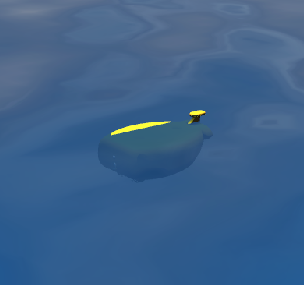
\includegraphics[width=.8\textwidth]{turbsim.png}
  \end{columns}
\end{frame}


%*----------- SLIDE -------------------------------------------------------------
\begin{frame}[c]{}
    %\transboxin[duration=1,direction=30]
    \centering
    %   \movie[width=12.8cm,height=7.2cm,showcontrols=true,poster,autostart]
    %         {\includegraphics[width=12.8cm,height=7.2cm]{Darwin-OP}}
    %         {Darwin-OP.mp4}


          %Videos and audios don't play on Overleaf! Download the PDF and open in Acrobat Reader to view. :-)

          %This is an .mp4 file:
          
          % using a .mp4; downloaded from https://www.youtube.com/watch?v=-9iXD2-hbJM
          %\includemedia[width=0.6\linewidth,height=0.6\linewidth,activate=pageopen,passcontext,transparent,addresource=penguinschasingbutterfly.mp4,flashvars={source=penguinschasingbutterfly.mp4}]{\includegraphics[width=0.6\linewidth]{penguins}}{VPlayer.swf}
          
          %This is a YouTube video (needs an Internet connection to view):
          
          % using a YouTube video
         % \includemedia[width=0.6\linewidth,height=0.3375\linewidth,activate=pageopen,flashvars={modestbranding=1 &autohide=1 autohide &showinfo=0 &rel=0}]{\includegraphics[width=0.6\linewidth]{Darwin-OP}}{https://www.youtube.com/v/g8Ejj0T0yG4?rel=0}
          
          %This is an .mp3 file:
          %% MP3 downloaded from https://www.sample-videos.com/download-sample-audio.php
        %   \includemedia[transparent,passcontext,addresource=SampleAudio.mp3,flashvars={source=SampleAudio.mp3},]{\color{blue}\framebox[0.4\linewidth][c]{Applause}}{APlayer.swf}

    \includemedia[
      width=.8\linewidth,
      totalheight=0.39375\linewidth,
      activate=pageopen,
      passcontext, 
      addresource=Media/movies/turbot_video_cut.mp4,
      flashvars={
      source=Media/movies/turbot_video_cut.mp4
      &autoPlay=true
      &Loop=false}
      ]{\fbox{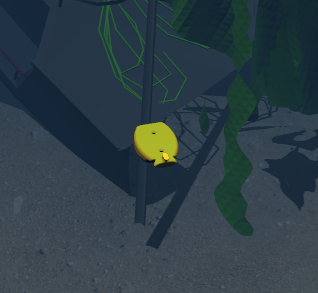
\includegraphics{turbot_intro}}}{VPlayer.swf}

    % \includemedia[
    %   width=.7\linewidth,
    %   totalheight=0.39375\linewidth,
    %   activate=pageopen,
    %   passcontext, 
    %   addresource=../Media/movies/turbot_video_cut.mp4,
    %   flashvars={
    %   source=../Media/movies/turbot_video_cut.mp4
    %   &autoPlay=true
    %   &Loop=false}
    %   ]{\fbox{}}{VPlayer.swf}

    %    \includemedia[
    %      width=0.4\linewidth,
    %      totalheight=0.225\linewidth,
    %      activate=pageopen,
    % %     passcontext,  %show VPlayer's right-click menu
    % %     addresource=Figures/Darwin-OP.mp4,
    %      flashvars={
    % %     %important: same path as in `addresource'
    % %     source=Figures/Darwin-OP.mp4}
    %         modestbranding=1 % no YT logo in control bar
    %         &autohide=1 % controlbar autohide
    %         &showinfo=0 % no title and other info before start
    %         &rel=0 % no related videos after end
    %         }
    %     ]{}{http://www.youtube.com/embed/1WEgNQjL66g}
    % %     &autoPlay=true
    % %     &Loop=false}
    % %     ]{\fbox{Click!}}{VPlayer.swf}

    %\pdfpcmovie{\includegraphics[width=.3\textwidth]{Darwin-OP}}{Darwin-OP.mp4}
%*----------- notes
    \note[item]{Notes can help you to remember important information. Turn on the notes option.}
\end{frame}
%-